% Unofficial Georgia Tech Psychology Poster Template
% based on
% https://github.com/k4rtik/uchicago-poster
% a fork of https://github.com/anishathalye/gemini

\documentclass[final]{beamer}
\fontsize{24pt}{28pt}\selectfont

% ====================
% Packages
% ====================

\usepackage[T1]{fontenc}
\usepackage{lmodern}
\usepackage{helvet}
\renewcommand{\familydefault}{\sfdefault}

% dimensions are in cm
\usepackage[size=custom, width=120, height=90, scale=1.2]{beamerposter}

\usetheme{gemini}
\usecolortheme{gatech}
\usepackage{graphicx}
\usepackage{booktabs}
\usepackage{doi}
\usepackage{natbib}
\usepackage[patch=none]{microtype}
\usepackage{tikz}
\usepackage{pgfplots}
\pgfplotsset{compat=1.18}
\usepackage{anyfontsize}
\usepackage{amsmath,bm}
\usepackage{enumitem}
\usepackage{amsmath}
\usepackage{amsthm}
\usepackage{amssymb}
\usepackage{mathtools}
\usepackage{amsbsy}
\usepackage{amssymb}
\usepackage{color}
\usepackage{xcolor}
\usepackage{tcolorbox}
\usepackage{mdframed}
\usepackage{arydshln}
\usepackage{caption}
\captionsetup{belowskip=3pt,aboveskip=3pt}

%%%%%%%%%% Custom Colors  %%%%%%%%%%%%%%
\usepackage[dvipsnames]{xcolor}

%% Mines Color
% The following are official colors for the Colorado School of Mines

\definecolor{paleBlue}{HTML}{CFDCE9}
\definecolor{lightBlue}{HTML}{879EC3}
\definecolor{blasterBlue}{HTML}{09396C}
\definecolor{darkBlue}{HTML}{21314d}
\definecolor{envrGreen}{HTML}{80C342}
\definecolor{goldenTech}{HTML}{F1B91A}
\definecolor{coloradoRed}{HTML}{CC4628}
\definecolor{lightGray}{HTML}{AEB3B8}
\definecolor{silver}{HTML}{81848A}
\definecolor{darkGray}{HTML}{75757D}
\definecolor{earthBlue}{HTML}{0272DE}
\definecolor{mutedBlue}{HTML}{57A2BD}
\definecolor{energyYellow}{HTML}{F0F600}
\definecolor{redFlannel}{HTML}{B42024}

%\newtheorem{theorem}{Theorem}
%\newtheorem{proposition}[theorem]{Proposition}
%\newtheorem{lemma}[theorem]{Lemma}
%\newtheorem{corollary}[theorem]{Corollary}
%\newtheorem{definition}[theorem]{Definition}
%\newtheorem{example}[theorem]{Example}
%\newtheorem{assumption}[theorem]{Assumption}
%\newtheorem{remark}[theorem]{Remark}
%\DeclareMathOperator*{\argmin}{\arg\!\min}

% defines spiffy box around examples

\newcommand{\T}{^{\rm T}}
\newcommand{\Cov}{{\rm Cov}}
\newcommand{\Cor}{{\rm Cor}}
\newcommand{\Var}{{\rm Var}}
\newcommand{\complex}{\mathbb{C}}
\newcommand{\real}{\mathbb{R}}
\newcommand{\naturals}{\mathbb{N}}
\newcommand{\integer}{\mathbb{Z}}
\newcommand{\indicator}{\mathbbm{1}}
\newcommand{\E}{\mathbb{E}}
\def\T{^{\rm T}}
\newcommand{\var}{var}
\newcommand{\cov}{cov}
\newcommand{\diag}{diag}
\newcommand{\tr}{tr}
\newcommand{\GP}{GP}
\newcommand{\avg}{avg}
\newcommand{\trace}{trace}
\newcommand{\blockdiag}{blockdiag}
\newcommand{\sign}{sign}
\newcommand{\knots}{\mathcal{Q}}
\newcommand{\grid}{\mathcal{G}}
\newcommand{\knot}{\mathbf{q}}
\newcommand{\likelihood}{\mathcal{L}}
\newcommand{\matern}{\mathcal{M}}
\newcommand{\node}{\mathcal{N}}
\newcommand{\normal}{\mathcal{N}}
\newcommand{\order}{\mathcal{O}}
\newcommand{\modu}{\mathcal{T}}
\newcommand{\Fourier}{\mathcal{F}}
\renewcommand{\prec}{\bm{\Lambda}}
\newcommand{\pprec}{\widetilde{\bm{\Lambda}}}
\newcommand{\domain}{\mathcal{D}}
\newcommand{\pp}{\omega}
\newcommand{\locs}{\mathcal{S}}
\newcommand{\sphere}{S}

\newcommand{\ba}{\mathbf{a}}
\newcommand{\bb}{\mathbf{b}}
\newcommand{\bc}{\mathbf{c}}
\newcommand{\bd}{\mathbf{d}}
\newcommand{\be}{\mathbf{e}}
\newcommand{\beff}{\mathbf{f}}
\newcommand{\bbf}{\mathbf{f}}
\newcommand{\bg}{\mathbf{g}}
\newcommand{\bh}{\mathbf{h}}
\newcommand{\bi}{\mathbf{i}}
\newcommand{\bj}{\mathbf{j}}
\newcommand{\bk}{\mathbf{k}}
\newcommand{\bl}{\mathbf{l}}
\newcommand{\bbm}{\mathbf{m}}
\newcommand{\bn}{\mathbf{n}}
\newcommand{\bo}{\mathbf{o}}
\newcommand{\bp}{\mathbf{p}}
\newcommand{\bq}{\mathbf{q}}
\newcommand{\br}{\mathbf{r}}
\newcommand{\bs}{\mathbf{s}}
\newcommand{\bt}{\mathbf{t}}
\newcommand{\bu}{\mathbf{u}}
\newcommand{\bv}{\mathbf{v}}
\newcommand{\bw}{\mathbf{w}}
\newcommand{\bx}{\mathbf{x}}
\newcommand{\by}{\mathbf{y}}
\newcommand{\bz}{\mathbf{z}}

\newcommand{\vep}{\varepsilon}
\newcommand{\vphi}{\varphi}

\newcommand{\sI}{\mathscr{I}}
\newcommand{\sR}{\mathscr{R}}
\newcommand{\sP}{\mathscr{P}}

\newcommand{\cD}{{\cal D}}
\newcommand{\cH}{{\cal H}}
\newcommand{\cP}{{\cal P}}
\newcommand{\cN}{{\cal N}}
\newcommand{\cS}{{\cal S}}
\newcommand{\cK}{{\cal K}}
\newcommand{\bA}{\mathbf{A}}
\newcommand{\bB}{\mathbf{B}}
\newcommand{\bC}{\mathbf{C}}
\newcommand{\bD}{\mathbf{D}}
\newcommand{\bG}{\mathbf{G}}
\newcommand{\bH}{\mathbf{H}}
\newcommand{\bI}{\mathbf{I}}
\newcommand{\bK}{\mathbf{K}}
\newcommand{\bL}{\mathbf{L}}
\newcommand{\bM}{\mathbf{M}}
\newcommand{\bP}{\mathbf{P}}
\newcommand{\bQ}{\mathbf{Q}}
\newcommand{\bR}{\mathbf{R}}
\newcommand{\bS}{\mathbf{S}}
\newcommand{\bT}{\mathbf{T}}
\newcommand{\bU}{\mathbf{U}}
\newcommand{\bV}{\mathbf{V}}
\newcommand{\bW}{\mathbf{W}}
\newcommand{\bX}{\mathbf{X}}
\newcommand{\bY}{\mathbf{Y}}
\newcommand{\bZ}{\mathbf{Z}}
\newcommand{\bomega}{\boldsymbol{\omega}}
\newcommand{\bbeta}{\boldsymbol{\beta}}
\newcommand{\bepsilon}{\boldsymbol{\epsilon}}
\newcommand{\bphi}{\boldsymbol{\phi}}
\newcommand{\bPhi}{\boldsymbol{\Phi}}
\newcommand{\blambda}{\boldsymbol{\lambda}}
\newcommand{\btheta}{\boldsymbol{\theta}}
\newcommand{\bvep}{\boldsymbol{\varepsilon}}
\newcommand{\bmu}{\boldsymbol{\mu}}
\newcommand{\bnu}{\boldsymbol{\nu}}

\newcommand{\bfzero}{\mathbf{0}}
\newcommand{\bfalpha}{\bm{\alpha}}
\newcommand{\bfgamma}{\bm{\gamma}}
\newcommand{\bfmu}{\bm{\mu}}
\newcommand{\bfxi}{\bm{\xi}}
\newcommand{\bftheta}{\bm{\theta}}
\newcommand{\bfeta}{\bm{\eta}}
\newcommand{\bfnu}{\bm{\nu}}
\newcommand{\bfrho}{\bm{\rho}}
\newcommand{\bfdelta}{\bm{\delta}}
\newcommand{\bfkappa}{\bm{\kappa}}
\newcommand{\bfbeta}{\bm{\beta}}
\newcommand{\bfepsilon}{\bm{\epsilon}}
\newcommand{\bftau}{\bm{\tau}}
\newcommand{\bfomega}{\bm{\omega}}
\newcommand{\bfpi}{\bm{\pi}}
\newcommand{\bfpsi}{\bm{\psi}}
\newcommand{\bfSigma}{\bm{\Sigma}}
\newcommand{\bfGamma}{\bm{\Gamma}}
\newcommand{\bfLambda}{\bm{\Lambda}}
\newcommand{\bfPsi}{\bm{\Psi}}
\newcommand{\bfOmega}{\bm{\Omega}}

\newcommand{\im}{{i_1,\ldots,i_m}}
\newcommand{\jm}{{j_1,\ldots,j_m}}
\newcommand{\jmp}{{j_1,\ldots,j_{m+1}}}
\newcommand{\jmm}{{j_1,\ldots,j_{m-1}}}
\newcommand{\jk}{{j_1,\ldots,j_k}}
\newcommand{\jl}{{j_1,\ldots,j_l}}
\newcommand{\jlp}{{j_1,\ldots,j_{l+1}}}
\newcommand{\jM}{{j_1,\ldots,j_M}}

\newcommand{\evol}{\mathcal{E}}
\newcommand{\levol}{\mathbf{E}}

\newcommand{\xp}{\mathbf{\widetilde{x}}} 
\newcommand{\yp}{\mathbf{\widetilde{y}}}
\newcommand{\xf}{\mathbf{\widehat{x}}}
\newcommand{\yf}{\mathbf{\widehat{y}}}

\newcommand{\Lp}{\mathbf{\widetilde{L}}}  
\newcommand{\Lf}{\mathbf{\widehat{L}}}  
\newcommand{\Sp}{\mathbf{\widetilde{S}}}  
\newcommand{\Sf}{\mathbf{\widehat{S}}}  

\newcommand{\ap}{\bm{\widetilde{\mu}}}     
\newcommand{\Pp}{\bm{\widetilde{\Sigma}}}  
\newcommand{\af}{\bm{\widehat{\mu}}}     
\newcommand{\Pf}{\bm{\widehat{\Sigma}}}  


\newcommand{\kronecker}{\raisebox{1pt}{\ensuremath{\:\otimes\:}}}

\newcommand{\bzero}{\boldsymbol{0}}
\newcommand{\bone}{\boldsymbol{1}}
\newcommand{\indep}{\perp \!\!\! \perp}

\pdfstringdefDisableCommands{%
\def\translate#1{#1}%
}

% ====================
% Lengths
% ====================

% If you have N columns, choose \sepwidth and \colwidth such that
% (N+1)*\sepwidth + N*\colwidth = \paperwidth
\newlength{\sepwidth}
\newlength{\colwidth}
\setlength{\sepwidth}{0.015\paperwidth}
\setlength{\colwidth}{0.3\paperwidth}

\newenvironment{myblock}
{\begin{tcolorbox}[colback=gray!10!white,colframe=gray!60!black]}
{\end{tcolorbox}}


\newcommand{\separatorcolumn}{\begin{column}{\sepwidth}\end{column}}
\newcommand{\bluebold}[1]{\textcolor{blue}{\textbf{#1}}}
\newcommand{\brownbold}[1]{\textcolor{brown}{\textbf{#1}}}



% ---------------------------- Poster Title ---------------------------$
\title{Example of Generic Mines Poster with Some Tips \\ to Use for Your Conferences!}


\author[Li et al.]{
  \underline{Ziyu Li}\inst{1} \and
  Blaster Donkey \inst{2} \and
  Daniel McKenzie \inst{1} \and
  Ore Digger\inst{3}
}
\institute{
  \inst{1} Applied Mathematics and Statistics, Colorado School of Mines;
  \inst{2} Hydrologic Science and Engineering, Colorado School of Mines;
  \inst{3} Geological Sciences, University of Alabama
}


%\institute[shortinst]{{Department of Applied Mathematics and Statistics, Colorado School of Mines}}

% ====================
% Footer (optional)
% ====================

\footercontent{
  \href{https://www.mines.edu/}{https://www.mines.edu} \hfill
  Colorado School of Mines, Golden, CO \hfill
  \href{mailto:ziyu_li@mines.edu}{ziyu\_li@mines.edu}}
% (can be left out to remove the footer)

% ====================
% Logo (optional)
% Change logos in the header by replacing the png files
% ====================


% ====================
% Body
% ====================

\begin{document}
\addtobeamertemplate{headline}{}
{
    \begin{tikzpicture}[remember picture, overlay]
      % Leftmost logo (Mines)
      \node (mineslogo) [anchor=north west, inner sep=3cm] at ([xshift=-0.5in, yshift=0.6in]current page.north west)
      {
\includegraphics[height=3.3in, width=3.3in]{Images/MinesLogo_WhiteBkg.png}};
      
      % New logo to the right of Mines
      \node [anchor=north west, inner sep=3cm] at ([xshift=3.5in, , yshift=0.6in]current page.north west)
      {
\includegraphics[height=3.3in]{Images/CIROHLogo_WhiteBkg.png}};
      
      % Rightmost logo (Alabama)
      \node [anchor=north east, inner sep=3cm] at ([xshift=0.5in, yshift=0.6in]current page.north east)
      {
\includegraphics[height=3.3in]{Images/UAlabama_WhiteBkg.png}};
    \end{tikzpicture}
}
\begin{frame}[t]
\begin{columns}[t]
\separatorcolumn

\begin{column}{\colwidth}

\begin{block}{Background}
\begin{itemize}[topsep=-4pt, partopsep=0pt, parsep=0pt, itemsep=4pt]
	\item[\large\color{blasterBlue}$\bullet$] Normally, you can add some exposition about your project here. 
	\item[\large\color{blasterBlue}$\bullet$] Use bullet points as much as possible. 
	\item[\large\color{blasterBlue}$\bullet$]  Cite your resources used, defined everything you need \cite{PlaceHolderSource}. 
	\item[\large\color{blasterBlue}$\bullet$] Here's how you write an equation that you can cite later:
	\begin{equation}
	\widehat{Q} = g^{\theta}(u, x, A),
	\label{eq:1}
	\end{equation}
	here, $g$ is \dots, $\theta = f^W(u, x, A)$, and $f$ are \dots  loss function $W = \text{argmin} \; L( Q, \widehat{Q})$. Define your variables!
\end{itemize} 

% add some vertical space. 
\vspace{0.5in}

If you would like to make a diagram, consider using free resources like \textcolor{redFlannel}{draw.io} or Power Point. And cite equation like this Equation \ref{eq:1}.
\begin{figure}[h]
	\centering
	
\includegraphics[width=\linewidth]{Images/NH-dCFEDiagram.png}
	\vspace{0.2in}
	\caption{Make sure you label your figures always using \texttt{label\{\}} function, so you can reference it later. Put figure captions here. }
	\label{fig:NH-dCFEDiagram}
\end{figure} 

\textbf{Usually, your problem statement or project goal will be around here. }
\end{block}

\begin{block}{Adjusting Size of Plots}
If you like Figure \ref{fig:NH-dCFEDiagram}, but want it smaller, you can change the \texttt{width} by scaling by \texttt{linewidth}. If no \texttt{height} variable was chosen, the aspect ratio will be kept. 
\vspace{0.25in}
\begin{figure}[h]
	\centering
	
\includegraphics[width=0.7\linewidth]{Images/NH-dCFEDiagram.png}
	\vspace{0.2in}
	\caption{Keep in mind resolutions of your plot and how visible it would be from afar.  }
	\label{fig:NH-dCFEDiagram_small}
\end{figure} 

\end{block}

 
\end{column}

\separatorcolumn
\begin{column}{\colwidth}
\begin{block}{PDF/SVG or PNG?}

\begin{center}
{\huge \textcolor{redFlannel}{\textbf{DO NOT SCREENSHOT PLOTS!}}}
\end{center}

Do not include pictures that are screenshots if possible. They usually do not scale well in a poster, and they can make you look less professional.  Ways to remedy this:

\begin{itemize}
	\item[\large\color{blasterBlue}$\bullet$] Use \texttt{pdf()} or \texttt{png()} in R. 
	\item[\large\color{blasterBlue}$\bullet$] Use \texttt{savefig()} or similar in Python to save as \texttt{.png} or \texttt{.pdf} or \texttt{.svg}. 
\end{itemize}

But PDFs/SVGs are generally preferred since they are vector based, but sometimes this doesn't make sense. 
\begin{figure}[h]
	\centering
	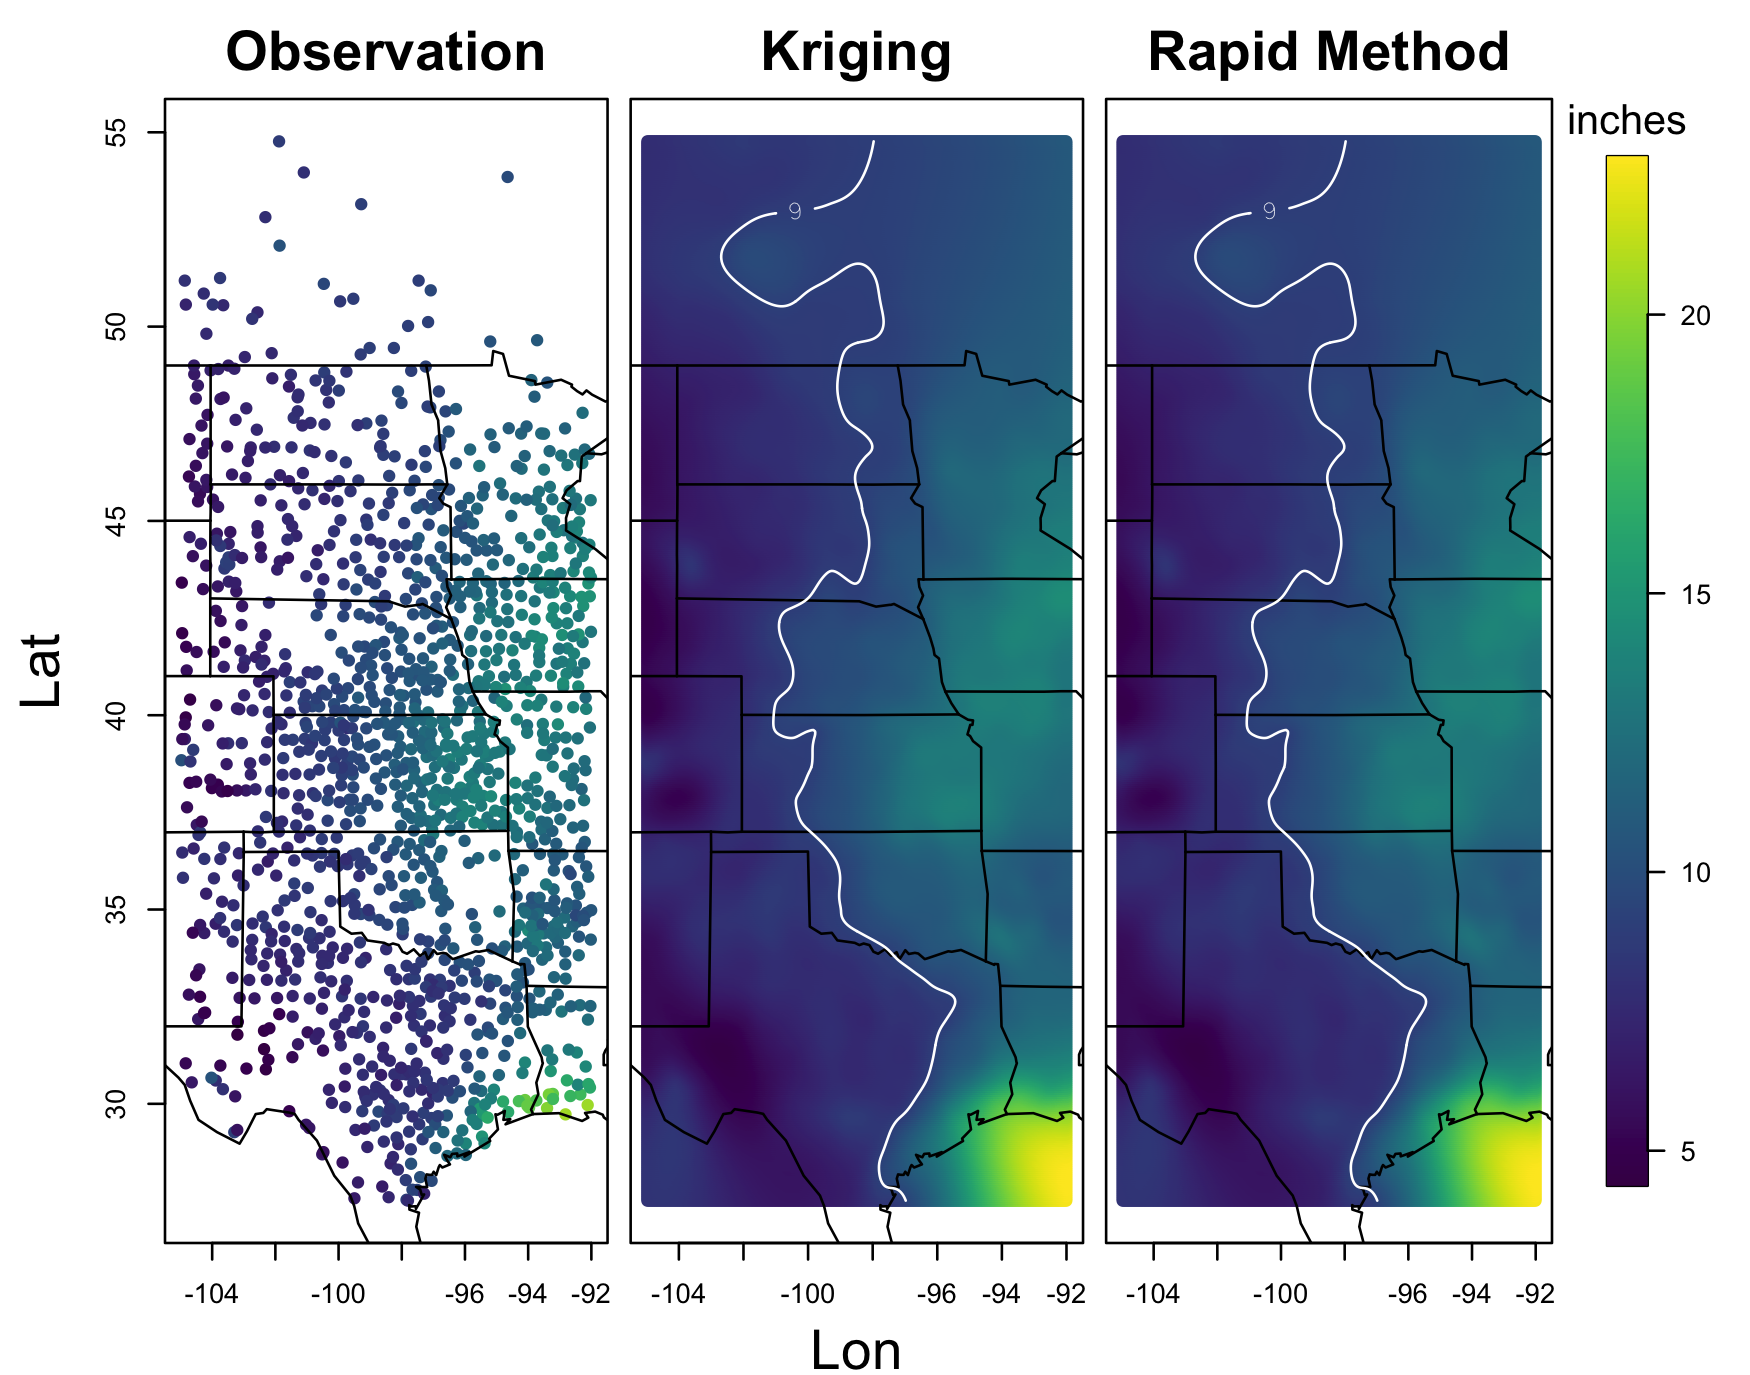
\includegraphics[width=0.75\linewidth]{Images/RainfallPredictionComparison_PosterVer_A.pdf}
	\caption{This plot is a pdf, and alone has the size of 11.7MB. This is because these are surfaces constructed by millions of individual points. }
	\label{fig:RainfallPDF}
\end{figure} 

% decrease space between plots. 
\vspace{-1cm}

\begin{figure}[h]
	\centering
	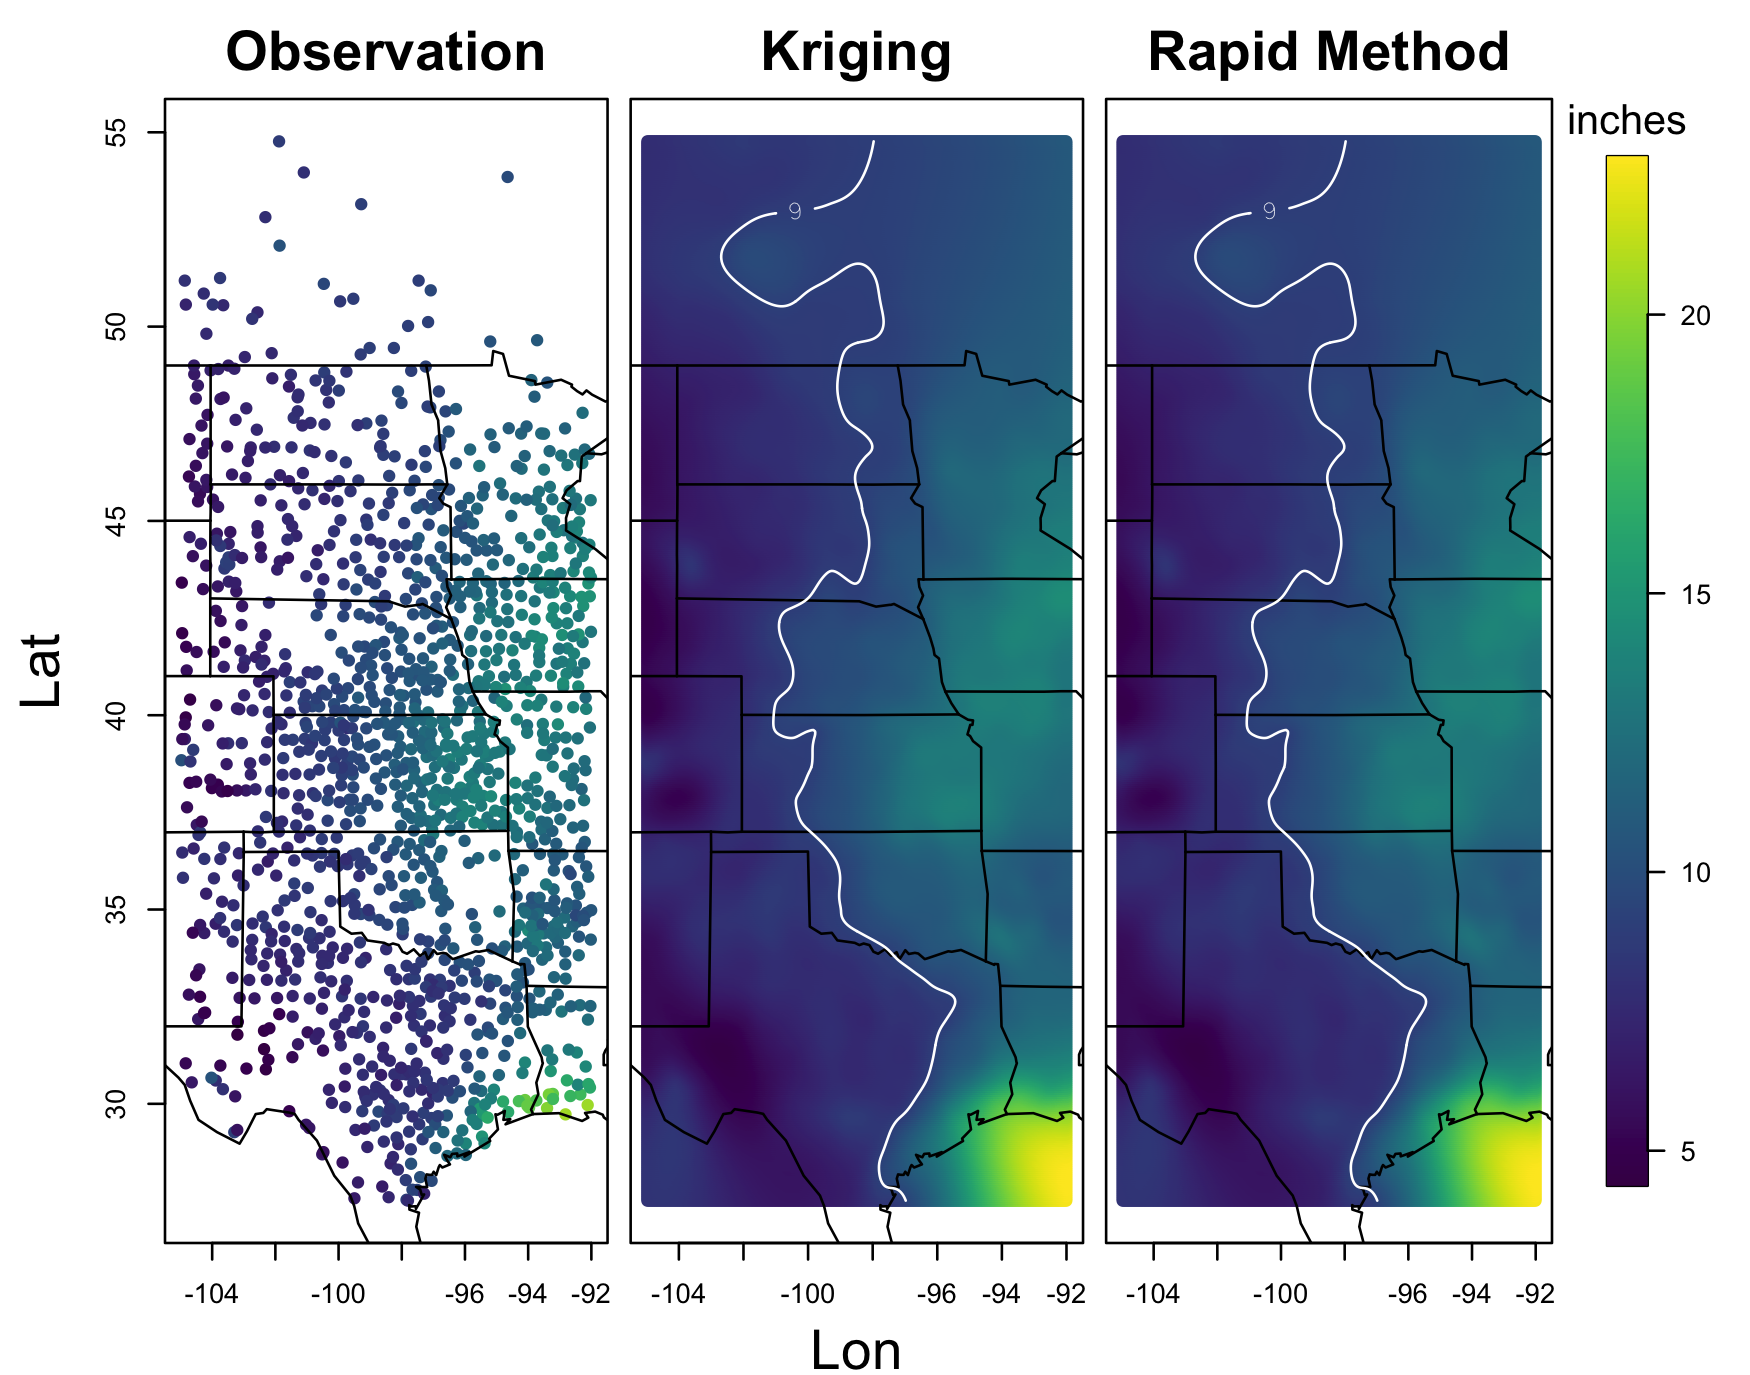
\includegraphics[width=0.75\linewidth]{Images/RainfallPredictionComparison_PosterVer_A.png}
	\caption{This plot is a png, and has the size of 1.2MB. Resolution can be adjusted to decrease file size more. }
	\label{fig:RainfalPNG}
\end{figure} 

\vspace{-1cm}

The PNG version is less vibrant but a lot smaller in size, which means it opens faster and less chances for corrupted files. Also, Mines print shop can only print items about less than 2MB (they lie on their website when they say 40MB), so you might not have a choice. 
\end{block}

\end{column}


\separatorcolumn
\begin{column}{\colwidth}

\begin{block}{PDF/SVG or PNG? Continued}

PDFs can sometimes be much more storage efficient. 
\begin{figure}[h]
	\centering
	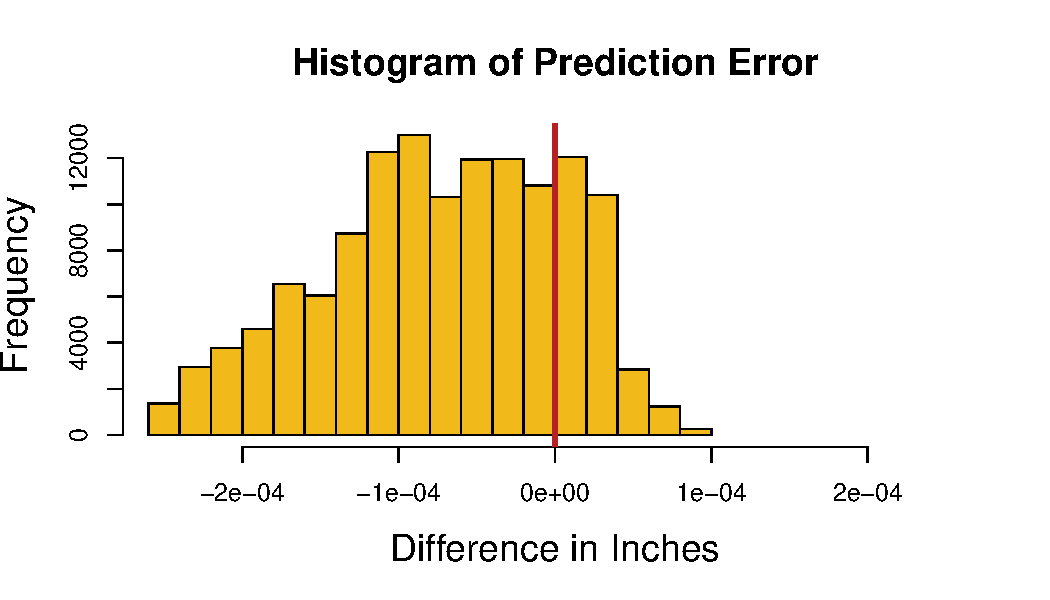
\includegraphics[width=0.9\linewidth]{Images/RainfallPredictionComparison_PosterVer_B.pdf}
	\caption{This plot is a pdf, and is 5kB in size.  The png version of this with similar resolution will be around 200 kB to start. }
	\label{fig:Histogram}
\end{figure} 

\end{block}

\begin{block}{Summary}
\textbf{How to write this part:}
	\begin{itemize}
		\item[\textcolor{blasterBlue}{\bullet}] Some advisors suggest a success/challenges summary. Some might do other formats. 		
		\item[\textcolor{blasterBlue}{\bullet}] But in general, you should summarize what you have achieved in your work and what is novel. 
		\item[\textcolor{blasterBlue}{\bullet}] Including any packages, papers etc. 
	\end{itemize}
\vspace{0.5cm}
\begin{columns}
 	\begin{column}{0.73\textwidth}
	\textbf{Splitting into 2 columns:}
\begin{itemize}
	\item[\textcolor{blasterBlue}{\bullet}] You can split this summary column into more columns to give you more creative freedom. 
	\item[\textcolor{blasterBlue}{\bullet}] This is how you do it. 
	\item[\textcolor{blasterBlue}{\bullet}] Be mindful on size of the plot and whatever you choose to put on the other side of it, they can look bad if not balanced correctly. 
	\end{itemize}
	\end{column}
	
	\begin{column}{0.25\textwidth}
	\begin{figure}[h]
	\centering
	
\includegraphics[width=\linewidth]{Images/MinesLogo_WhiteBkg.png}
	\caption{Mines logo}
	\label{fig:Mines}
\end{figure} 
	\end{column}
\end{columns}

\end{block}

\begin{block}{Future Work}
\begin{itemize}
	\item[\textcolor{blasterBlue}{\bullet}] Put something here.
	\item[\textcolor{blasterBlue}{\bullet}] Refine code.... 
	\item[\textcolor{blasterBlue}{\bullet}] Something else
\end{itemize}
You might need to compile this with LuaLaTeX. 
\end{block}

\begin{block}{References}
%\nocite{*}
\footnotesize{\bibliographystyle{abbrv}\bibliography{Sources}}
\end{block}
\end{column}

\separatorcolumn
\end{columns}

\end{frame}
\end{document}